\chapter[Primate Phylogenetics with Landmark Data]{Primate Phylogenetics with Landmark Data: \\Exploring Model-Based and Heuristic Approaches}

\label{chpt:Chapter3}

\chapterauthor{Nikolai G. Vetr, Timothy D. Weaver}

\clearpage

\section{Abstract}

Paleontologists and paleoanthropologists have long sought to better understand evolutionary relationships linking fossil and extant taxa. While modern genetic and genomic methods offer ample opportunity for phylogenetic inference, age and degradation quickly limit adequate retrieval of ancient DNA from fossil specimens. New approaches extending phylogenetic models common in the comparative methods literature could conceivably improve inference of fossil phylogeny over more commonly used heuristic methods developed prior to recent decades' advances in computation and theory. Here, we explore the application of a stochastic multivariate Brownian diffusion model to a set of landmark data collected across a range of catarrhine primate species. We contrast results from this fitted model to those obtained from Bayesian analysis of matched molecular data, as well as to results from more conventional, heuristic inference procedures, such as distance-based methods and Maximum Parsimony. A short simulation study is also performed to explore the behavior of the multivariate Brownian method under empirically parameterized conditions. With the advent of increasingly sophisticated continuous character data capture technologies, improved understanding of how different methods perform will help to inform researchers' phylogenetic analyses and better infer the evolutionary relationships connecting both fossil and extant taxa. [Primate Evolution; Bayesian Inference; Multivariate Brownian Motion]

\clearpage

\section{Introduction}

Phylogenies are inferred representations of the branching process of speciation, the splitting of ancestral populations into reproductively isolated daughter lineages. Evolution makes little sense except in their light. But far from merely depicting genealogical relationships among taxa of interest, their inference is essential to the investigation of many evolutionary questions. Perhaps most importantly, they serve as a scaffold for the analysis of character evolution \citep{felsensteinPhylogeniesComparativeMethod1985}, as shared ancestry confounds relationships between traits observed in taxa evolving along the branches of phylogenetic trees. They also provide a framework for divergence time estimation \citep{glazkoEstimationDivergenceTimes2003, heathBayesianInferenceSpecies2014}, ancestral trait reconstruction \citep{schluterLikelihoodAncestorStates1997, joyAncestralReconstruction2016}, species delimitation and taxonomic classification \citep{rannalaArtScienceSpecies2015}, historical biogeography \citep{donoghueIntegrativeHistoricalBiogeography2003, ronquistPhylogeneticMethodsBiogeography2011}, analysis of lineage diversification \citep{neeReconstructedEvolutionaryProcess1994, morlonPhylogeneticApproachesStudying2014}, and much more. They can help to generate, constrain, and discriminate between paleontological hypotheses, guiding our interpretation of the fossil record. Whether some species is ancestor, sister, or descendant to some other species; whether the same character evolved many times, convergently, or just once; whether suites of characters coevolved simultaneously or appeared piecewise; these and other questions can be explicitly explored within a phylogenetic framework. 

Likely owing to our own taxonomic affinities and the wide availability of both morphological and molecular data, primates -- especially the catarrhine primates --  serve as a common target for the application of new phylogenetic methods or the exploration of existing methods \citep[e.g.][]{reisUsingPhylogenomicData2018} and as examples in tutorials demonstrating the use of phylogenetic software (e.g. in Beast or RevBayes; \citealt{bouckaertBEASTAdvancedSoftware2019}; \citealt{hohnaRevBayesBayesianPhylogenetic2016a}). Though most recent analyses of primate phylogeny focus on molecular data \citep[e.g.][]{perelmanMolecularPhylogenyLiving2011, springerMacroevolutionaryDynamicsHistorical2012}, historical attempts at inference made use primarily of morphological characters, despite their arguable unreliability at retrieving trees compatible with molecular results \citep[e.g.][]{collardHowReliableAre2000, gibbsSofttissueCharactersHigher2000, varon-gonzalezEstimatingPhylogeniesShape2020}. When inferring phylogeny among fossil taxa, paleontologists are often limited to the use of morphological characters, as degradation quickly limits the ages of fossils from which ancient DNA can be successfully extracted, sequenced, and assembled \citep{collinsSurvivalOrganicMatter2002, allentoftHalflifeDNABone2012, pickrellNewHistoryGeography2014}. Among hominins, for example, attempts to infer phylogeny have made use of a panoply of algorithms -- described briefly below -- to transform some alignment of morphological character data into a point estimate or set of phylogenetic trees. There exists a long history of these attempts, stretching many decades into the past \citep[e.g.][]{chamberlainEarlyHominidPhylogeny1987, stringerNumericalCladisticAnalysis1987, skeltonEvolutionaryRelationshipsEarly1992, straitReappraisalEarlyHominid1997}, but also in recent years \citep[e.g.][]{irishDentalMorphologyPhylogenetic2013, demboBayesianAnalysisMorphological2015, demboEvolutionaryRelationshipsAge2016, argueAffinitiesHomoFloresiensis2017}. To further inform practice in these contexts, it is useful to explore the performance of newer, model-based methods for inferring phylogeny using morphological characters, contrasting their output with results from more conventional approaches, such as Maximum Parsimony or distance-based methods. A natural system for such a comparison can be found, of course, in the catarrhine primates.

The most popular inference model for phylogenetically structured morphological data is Lewis’ (\citeyear{lewisLikelihoodApproachEstimating2001}) Mk-model, which can be fit in both Bayesian and Maximum Likelihood frameworks. For four-state characters, it is identical to the Jukes-Cantor (\citeyear{jukesEvolutionProteinMolecules1969}) model of nucleotide substitution (as the canonical state-space of DNA is 4), and otherwise generalizes the Jukes-Cantor model to arbitrary numbers of states. This model is well explored in phylogenetic contexts, both in the nucleotide substitution case and for discrete morphological characters \citep[e.g.][]{wrightModelingCharacterChange2016}. Fitting this model under maximum likelihood produces a point estimate of tree topology, branch lengths, and evolutionary model parameters that corresponds to the parameter values under which the observed data are most plausible (the Maximum Likelihood Estimate, or MLE). Conversely, the Bayesian target of inference is the entire joint posterior distribution of phylogenetic model parameters, often approximated numerically with Markov chain Monte Carlo (MCMC).

Other phylogenetic inferential methods commonly applied to morphological datasets include tree-search under the Maximum Parsimony (MP) criterion and some cost matrix, as well as clustering algorithms (e.g. neighbor joining or UPGMA) that accept as input some distance matrix and produce as output a tree with particular properties. Both typically also produce point estimates, though one can envision procedures (e.g. the non-parametric bootstrap; \citealt{efronBootstrapMethodsAnother1979}; \citealt{felsensteinConfidenceLimitsPhylogenies1985}) that incorporate sampling or measurement uncertainty, as one might also do with Maximum Likelihood inference. For MP methods, often there can be obtained a set of distinct most parsimonious or nearly-most parsimonious trees, but how one probabilistically interprets the frequency of clade membership in this set is unclear. Parsimony can also mislead under certain conditions even at the limit of infinite data, such as when evolutionary rates are high or heterogenous \citep{wrightBayesianAnalysisUsing2014, wrightModelingCharacterChange2016, oreillyProbabilisticMethodsSurpass2018}, and typically requires the use of independent, discrete characters. Distance methods can calculate distances that incorporate evolutionary models of character change, but also struggle to accommodate inferential uncertainty in a principled manner, especially in a multivariate framework where resampling characters cannot, by construction, supply any further phylogenetically meaningful information. 

Frequently, morphological variation between groups is not discrete, but continuous. While distances can easily be computed between sets of continuous characters, inference under the Mk-model \citep{lewisLikelihoodApproachEstimating2001} and most parsimony-based methods \citep{goloboffContinuousCharactersAnalyzed2006} often require that we discretize any continuous observations. Continuous forms of MP algorithms do exist, such as Squared-Change Parsimony \citep{maddisonSquaredchangeParsimonyReconstructions1991, rohlfGeometricMorphometricsPhylogeny2002}, Linear Parsimony \citep{klugeQuantitativePhyleticsEvolution1969}, Manhattan-Metric Parsimony \citep{swoffordInferringEvolutionaryTrees1987}, and others \citep[see][]{rogersComparisonSuitabilityRogers1991}, but these are almost always applied to quantitative characters in the service of ancestral state reconstruction and not the inference of tree structure itself, and so will not be directly considered here. Discretization can be done in a variety of ways \citep{garcia-cruzCodingQuantitativeCharacter2006, thorpeCodingMorphometricCharacters1984} in part subject to researcher preference, with some methods retaining more phylogenetic information than others \citep{brazeauProblematicCharacterCoding2011, worthingtonSelectionCharacterCoding2017}. Even discrete characters collected at the outset may just be discretizing some fundamentally quantitative feature \citep{wiensCharacterAnalysisMorphological2001}, relying on a researcher's present observations and prior experiences instead of an explicit algorithm run on the character alignment in its entirety. Recent decades have also witnessed the rise of new techniques for the collection of continuous morphological data, such as surface and CT scanning \citep{mitteroeckerAdvancesGeometricMorphometrics2009, adamsFieldComesAge2013, reinGeometricMorphometricsVirtual2014}. As such, we may desire to better understand statistical methods for inferring phylogeny that can make direct use of continuous characters without needing to discretize them. 

Inference under a multivariate Brownian motion model of character evolution may satisfy this desire. Multivariate Brownian motion (mvBM) is a straightforward extension of univariate Brownian motion \citep{felsensteinMaximumlikelihoodEstimationEvolutionary1973}, modifying only that displacements to character states be drawn from multivariate normal distributions, rather than univariate normal distributions. This allows for the representation of phenomena such as pleiotropy, correlated selection, linkage, and integration, which may structure the evolution of quantitative traits. Here, we investigate how well an mvBM model fit in a Bayesian statistical framework is able to retrieve catarrhine phylogeny using 15 3-Dimensional craniofacial landmarks sampled across a collection of 13 catarrhine primate species \citep{harvatiNeanderthalTaxonomyReconsidered2004}. We compare this inference to those obtained from other parametric models of character evolution, both distance-based and Maximum Parsimony methods, as well as to relationships in this group inferred from molecular data \citep{arnold10kTreesWebsiteNew2010}. We then perform a short, empirically realistic simulation study under mvBM to explore the performance of the method in its ability to retrieve true, data-generating trees and clades when the inference model is well specified. 

\clearpage

\section{Materials and Methods}

Empirical data used in this analysis were drawn from the (\citeyear{harvatiNeanderthalTaxonomyReconsidered2004}) work of Harvati and colleagues and consisted of 15 3-dimensional craniofacial landmarks sampled on 13 species of catarrhine primate. Samples were also partitioned at the subspecific level, with 7 populations of \textit{Homo sapiens}, 6 subspecies of \textit{Papio hamadryas}, 3 subspecies of \textit{Pan troglodytes}, and 2 subspecies of \textit{Gorilla gorilla} present in the dataset, for 27 total tips at maximum taxonomic resolution. Given the extent of hybridization known to occur between subspecies and populations --- for example, in \textit{Papio hamadryas} \citep{rogersComparativeGenomicsComplex2019} --- we lumped together all divisions in the data below the species level, that their phylogeny might be better represented by a non-reticulate, strictly bifurcating tree. Sample sizes for extant species ranged from 17 for \textit{Macaca hecki} to 400 for \textit{Papio hamadryas}; the only extinct species in the analysis, \textit{Homo neanderthalensis}, was also present in the fewest number, with 5 sampled individuals. Information regarding the composition of this dataset can be found in Table \ref{tab:landmarkDataComposition}, with more information on the precise sample composition and locations of specific landmarks able to be found in the aforementioned paper \citep{harvatiNeanderthalTaxonomyReconsidered2004}. These data also contained information on each individual's estimated sex, and to avoid the confounding effects of sexual dimorphism we treated sex-specific observations as representing separate, independently evolving partitions, pooling information across partitions with respect to topology but otherwise independently estimating phylogenetic model parameters. In other words, we specified an evolutionary model where male and female morphologies were able to evolve independently from one another, constrained only in that the branching order of speciation events had to be identical for both. Given the non-independent nature of within-species male and female morphology, this may induce some degree of pseudo-data-duplicatory effect, but additional pooling of model parameters was judged inappropriate given further transformations described below.

This dataset has several features that make it desirable for the analyses performed here. The species included are not only highly studied but also of intrinsic interest, with well ascertained molecular phylogenies available for comparison. Additionally, the landmark nature of the data makes exploring the statistical performance of modern multivariate phylogenetic methods especially enticing, given the projected proliferation of these datasets as morphologists continue to develop semiautomated landmark capture techniques. Past attempts to infer phylogeny using craniofacial morphology have met mixed success \citep[e.g.][]{collardHowReliableAre2000}, so assessing the performance of different methods with respect to both empirical and simulated data may help to inform researchers' decisions when analyzing landmark data from other systems. 

Before the data could be analyzed, several pre-processing steps were required. First, we performed Procrustes transformation \citep{gowerGeneralizedProcrustesAnalysis1975, drydenStatisticalShapeAnalysis2016} on all data irrespective of sex simultaneously, scaling the set of each individual's landmarks to unit centroid size and iteratively rotating and translating until the Procrustes distances across all individuals' landmarks converged to some minimum value \citep{booksteinLandmarkMethodsForms1997}. This was done using the \texttt{gpagen()} function in the \textit{geomorph} package \citep{adamsGeometricMorphometricAnalyses2019} in \textit{R} \citep{rcoreteamLanguageEnvironmentStatistical2013}. Following Mitteroecker and colleagues (\citeyear{mitteroeckerComparisonCranialOntogenetic2004}) and to allow size and not just shape to inform subsequent analyses, log-centroid size was reintroduced as a single additional variable, bringing the total number of traits used to 46 (3 x 15 shape coordinates + size). 

However, the evolution of these 46 traits is not independent, and so we might attempt to correct for this nonindependence before attempting any phylogenetic analysis. To do this, we compute the sex-specific pooled within-group covariance matrix of our transformed landmark data, $P$. Under Cheverud's conjecture \citep{cheverudDevelopmentalIntegrationEvolution1996}, this should be proportional to the additive genetic covariance matrix, $G$, which describes the variances and covariances of morphological evolution at mutation-drift equilibrium \citep{weaverNeutralTheoryEvolution2018a}. However, as Procrustes transformation removes 7 degrees of freedom (1 for translation and rotation in each of the three dimensions, 1 for scaling), the resulting $P$ matrix is rendered non-positive-semidefinite --- with seven negative eigenvalues trailing --- and therefore uninvertible, which makes it unsuitable for use in, for example, an informative prior for the multivariate Brownian motion rate matrix. To circumvent this limitation, we decompose P into its eigensystem, with columns of the eigenvector matrix ordered according to monotonically decreasing eigenvalues. We then project the Procrustes transformed landmarks onto those eigenvectors corresponding only to the positive eigenvalues, and further divide them by the square root of each corresponding eigenvalue, effectively transforming the 46 original characters into 39 whose pooled within-group covariance matrix equals the identity matrix. As a further dimensionality reduction step, we examine the scree plot of our eigensystem and discard those later axes comprising the final 1\% of the total variance, restricting ourselves to the minimum set of axes corresponding to 99\% of the total within-group variance, and reducing the number of characters to be analyzed to 19 in the female partition and 20 in the male. Thus, subsequent analyses assume that evolution can only occur within a lower dimension subspace along these principal axes, which do not span the entire space of our 46 characters, but may nevertheless allow for it to realize most of the variation observed in the empirical data. We relax this assumption and allow for greater non-independence in the Brownian motion model, but otherwise treat these normalized scores as independent outcomes of the evolutionary data-generating process.

To incorporate information from both sexes into the heuristic analyses performed here, we were not able to specify separate data partitions with greater or lesser degrees of parameter pooling, as heuristic methods lack a formal description of the data-generating process. Instead, we treated scores on each of the axes as independent observations for each tip, concatenating them into a single morphological character alignment.

Finally, no female Neandertals were present in the morphological dataset. To allow for the joint analysis of both partitions in phylogenetic software, we required equality between the sets of tips in either partition. Preliminary male-specific analysis found that Neandertals and \textit{Homo sapiens} clustered together with high confidence regardless of method or model used, so to construct a fictitious female Neandertal we found the vector difference between the two species means of male genus \textit{Homo} and displaced the female \textit{Homo sapiens} mean by that difference. This was done after the joint Procrustes transformation but before projection of species means onto each respective $P$'s eigenvectors, with the fictitious female Neandertal then projected onto the female $P$'s eigenvectors and included in the female partition for analysis.

Some methods required additional pre-processing, the details of which can be found below. In total, we inferred catarrhine phylogeny using three heuristic methods: UPGMA, Neighbor-Joining, and Maximum Parsimony; as well as under four models in a Bayesian framework: univariate Brownian motion, multivariate Brownian motion, Lewis' Mk model, and an ordered Continuous Time Markov Chain (CTMC) model. Each is described in turn. 

\subsection{Distance-Based Methods}

Two clustering algorithms served our purposes here -- the Unweighted Pair Group Method with Arithmetic mean algorithm \citep{sokalStatisticalMethodEvaluating1958} and the Neighbor-Joining algorithm \citep{saitouNeighborjoiningMethodNew1987}. Both were implemented in R as the functions \texttt{upgma()} and \texttt{nj()} in the \textit{phangorn} \citep{schliepPhangornPhylogeneticAnalysis2011} and \textit{ape} \citep{paradisAPEAnalysesPhylogenetics2004} packages, respectively. These methods require that we provide them a distance matrix, which they then use to construct either a rooted ultrametric tree or an unrooted tree with identical patristic distances (with elements of the distance matrix equal the sums of branch lengths separating tips). To compute a distance matrix, we needed a measure of distance between pairs of taxa. For this, we used the Euclidean distances between our transformed traits, similar to using a squared Mahalanobis distance \citep{mahalanobisGeneralizedDistanceStatistics1936} with $P$ serving to standardize distances between tips, as under our transformation of the character data, $P$ became the identity matrix. 

\subsection{Data Discretization}

Both the maximum parsimony analyses and many popular parametric evolutionary models require that data be discrete, rather than continuous. A number of approaches were available here, and we explored two. For the first, we followed the divergence coding procedure favored by Collard and Wood (\citeyear{collardHowReliableAre2000}, \citeyear{collardHowReliableAre2001}) and described by Thorpe (\citeyear{thorpeCodingMorphometricCharacters1984}). This assigned each tip a discrete character in the range ($1, 2, ..., 2n_{tips} - 1)$) and may better accommodate differences in the spacing between tips along a continuous scale, with larger differences corresponding to greater required amounts of evolutionary change. Conversely, the second discretized our continuous character ranges into intervals according to Jenks Natural Breaks Optimization Method \citep{jenksDataModelConcept1967}, implemented via the \texttt{classIntervals()} function in the \textit{classInt} package \citep{bivandPackageClassInt2020} in \textit{R}. Jenks' algorithm identifies a pre-specified number of breakpoints along a continuous distribution so as to optimally divide that distribution into categories such that total within-category variance is minimized. As a compromise between flexibility and computational convenience, we set a threshold Goodness of Variance Fit (GVF) value such that the average number of categories across traits was closest to four. This allowed different traits to have different numbers of categories, depending on their need for them. If a character could be discretized into two or three states and exceed the requisite GVF, it could effectively ``donate" its opportunity for further discretization to a different character not yet meeting the threshold.

\subsection{Maximum Parsimony}

Maximum Parsimony based methods describe a set of algorithms that explore tree-space in search of a tree that minimizes the amount of evolutionary change needed to produce some observation of character data. Typically, evolutionary change is represented in a parsimony score that measures the smallest number of discrete steps compatible with a given discrete character alignment, and taking Collard and Wood (\citeyear{collardHowReliableAre2000}) for inspiration, we performed inference under the maximum parsimony criterion using traits discretized under divergence coding.

To search for the optimally short tree, we used the Parsimony Ratchet \citep{nixonParsimonyRatchetNew1999}, implemented as the \texttt{pratchet()} function in the \textit{phangorn} package in \textit{R}. Given the ordinal nature of divergence-coded traits, we also supplied a Wagner Cost Matrix whose entries $W_{i,j}$ corresponded to the absolute value of the difference between the $i^{th}$ row and $j^{th}$ column, representing the penalty to the parsimony score of particular transitions (e.g. moving from state 25 to state 13 would contribute a penalty of $25 - 13 = 12$ to the parsimony score). As the parsimony ratchet may be susceptible to capture by local minima, we ran it 50 times from independent starting trees (generated with the \texttt{rtree()} function in \textit{ape}), recording the final state of each chain after 500 iterations had passed without the discovery of a lower-scoring tree. The shortest tree or set of trees across these replicates was taken to be the global minimum.

\subsection{Bayesian Inference}

Four evolutionary models were assumed for the Bayesian analyses performed in \textit{RevBayes}, which uses the Metropolis-Hastings algorithm, a form of Markov chain Monte Carlo (MCMC), to approximate the joint posterior distribution of phylogenetic model parameters. These models include the univariate and multivariate Brownian motion model of continuous character evolution, the Mk-model --- which generalizes Jukes-Cantor --- and an ordered Continuous Time Markov Chain model with equal instantaneous rates of change between adjacent states and rates of 0 elsewhere. These models were used to analyze the transformed landmark data in the case of uvBM and mvBM, and the Jenks-coded traits in the case of the two CTMC models.

In the Brownian motion analyses, we specified an informative prior on the multivariate Brownian rate matrix about the identity, effectively centering it around the empirical $P$, as expected under neutrality or fluctuating selection by quantitative genetic theory. In the multivariate Brownian analysis, we set independent priors on the correlation and variance components of the rate matrix, with an LKJ($\eta = 20$) for the former and a Dirichlet multiplied by the number of characters in each partition for the later. This had the effect of fixing the \textit{average} rate of each rate matrix to one, allowing their identifiability when also attempting to estimate branch lengths. A log$_{10}$normal(1, 0.25) + 1 offset hyperprior was placed on the concentration parameters of this Dirichlet distribution to adaptively regularize the degree of rate heterogeneity along each principal component while still specifying an \textit{a priori} preference towards equal rates, relaxing slightly the Cheverud's conjecture assumption. In the \textit{univariate} Brownian analysis, we fixed the correlation component of the rate matrix to the identity, inferring only the diagonal variances, or rates. Strictly speaking, this latter analysis does not represent a univariate Brownian motion over the original landmark data, but rather corresponds to one involving simultaneously greater or lesser degrees of correlation and rate in the traits that load more on each eigenvector. When the estimated rate matrix is precisely the identity, the implied rate matrix is equal to P, to the extent that it is well approximated by recomposition using only those first eigenvectors corresponding to 99\% of the sum of the eigenvalues. The multivariate Brownian analysis, meanwhile, allows for finer-tuned inference of trait correlations and rates in directions not reflected by the eigenvectors of P. A discrete uniform prior was specified for the topology parameter, a log$_{10}$normal(1, 1) prior for the overall tree length, and a flat Dirichlet(1,1,1,...) for the branch length proportions. 

%Rather than apply a further transformation to the data and risk violating Brownian assumptions, we instead found the nearest positive-semidefinite covariance matrix following the iterative algorithm described by Higham (\citeyear{highamComputingNearestCorrelation2002}) and implemented in the \textit{R} package \textit{Matrix} \citep{batesPackageMatrix2019}. The effect of this operation was minute: the largest change experienced by any element of the correlation matrix was on the order 3E-7. 

Following convention \citep{yangAmongsiteRateVariation1996}, we allowed gamma-distributed among site rate variation (ASRV) in the CTMC models, approximated by averaging over 4 discrete rate categories specified according to equally spaced quantiles and fixing both of the gamma's shape parameters to equality (thereby constraining the mean rate to be 1). A log$_{e}$normal(e, 1) prior was used for the one shape parameter of our gamma-ASRV model. The same lognormal and flat Dirichlet priors for tree length and branch length proportions were used here as for the mvBM analysis.

Analyses under mvBM and the Mk-models were run for 20,000 iterations in each of two independently seeded chains, with a preceding 5,000 iterations discarded as burn-in and used for proposal distribution tuning. Each iteration consisted of 5,370 proposals. Thus, analyses were run for 26,850,000 moves each. Metropolis-coupling \citep{geyerMarkovChainMonte1991, altekarParallelMetropolisCoupled2004} with one heated chain was used to improve mixing. 

A number of diagnostics were used to diagnose the health of MCMC output. Beyond terminal branch lengths, tree length, the computed likelihood value, and the posterior density, the pairwise correlations, trait-specific rates, and all regularizing hyperparameters, several ``fictitious" parameters were coerced from the Newick strings recorded by \textit{RevBayes}. These included patristic distances between all of pairs of tips, Robinson-Foulds (RF; \citeyear{robinsonComparisonPhylogeneticTrees1981}) and Kuhner-Felsenstein (KF; \citeyear{kuhnerSimulationComparisonPhylogeny1994}) distances from an arbitrary reference tree, and the presence or absence of the twenty most common bipartitions with frequency $< 0.99$. Visual inspections of marginal histograms, rank plots, trace plots, compare-trees plots, and multidimensional scaling plots were performed at first pass; then, effective sample sizes were computed using the \texttt{effectiveSize()} function in the \textit{R}-package \textit{CODA} \citep{plummerCODAConvergenceDiagnosis2006} and ensured to fall above 500 for each real and generated parameter, using first each independent chain and then both concatenated. Additionally, R$^2$ values for all bipartition frequencies in either chain above 0.01 were required to fall above 0.95. 

\subsection{Inverse Analysis}

In a follow-up analysis, we explored the inverse problem --- given a time-calibrated phylogeny of these 13 catarrhine species and their 45 Procrustes-transformed landmarks and log-centroid size, to what extent do we see morphological evolutionary rate variation in the mvBM process, and how well does the pooled within-group covariance matrix approximate the inferred multivariate Brownian motion rate matrix? Here, we require a well-ascertained, preferably time-calibrated phylogeny of those taxa present in the morphological dataset. Rather than conduct such an analysis ourselves, we instead relied upon trees drawn from the \emph{10kTrees Project} online repository \citep{arnold10kTreesWebsiteNew2010}, which will also serve as an external check on method reliability. These represent samples drawn from the joint posterior of a Bayesian analysis of primate phylogeny performed on 17 nuclear and mitochondrial genes under a partitioned scheme of GTR-family models selected by \emph{JModelTest} \citep{posadaJModelTestPhylogeneticModel2008}. All taxa included in the Harvati dataset were present here up to species designation, with only one subspecies --- the Kinda baboon, \emph{Papio hamadryas kindae}, absent, so we subsetted the dataset to include only those species for whom morphological data was present. Then, we generated a Maximum Clade Credibility (MCC) tree via \textit{phangorn} \citep{schliepPhangornPhylogeneticAnalysis2011} for these molecular trees, conditioning on it for this follow-up analysis. On this tree we fit an uncorrelated relaxed morphological clock model with parameterization similar to that used to infer topology earlier, involving a flat LKJ($\eta = 1$) prior on the correlation component of the rate matrix, a Dirichlet prior on the relative variance components with log$_{10}$normal(0,1) + 1 hyperprior on its concentration parameters, scaled by the number traits that the average rate equal 1, a log$_{10}$normal(1,1) prior on the total branch-specific rates, and another Dirichlet prior with log$_{10}$normal(0,1) + 1 hyperprior on the concentration parameters to multiply the total branch-specific rates and obtain individual branch-rates. Independent analyses were performed on the male and female tips in the sample, so we did not include the fictitious female Neandertal tip in the female analysis. Four independent, Metropolis-coupled chains were run with 1 heated and 1 cold chain each to achieve adequate sampling, and all the aforementioned MCMC diagnostics applied to model parameters including branch rates, with the exception of those involving tree topology and branch lengths, as both were fixed in these analyses. 

\subsection{Simulation Experiment}
To help identify the degree to which the error observed in these analyses could be expected or else attributed to model misspecification or the various transformations we performed in the name of tractability or convenience, we performed a short simulation experiment in which 46 x 2 = 92 characters were simulated to evolve under multivariate Brownian motion on the time-calibrated MCC tree obtained from the \emph{10kTrees Project}. Branch rates and mvBM rate matrices were drawn from the posterior distribution of the Inverse Analysis described above. To simulate the pseudoreplication inherent to treating male and female tip means as outcomes of independent data-generating process, we averaged sampled rate matrices $R_{F}$ and $R_{M}$ to obtain a single matrix, $R_{MF}$, which we Kronecker multiplied by a 2 x 2 correlation matrix with off-diagonal 0.9, used to represent the coincident evolutionary trajectories of each sex within the same evolutionary lineage. This procedure induced strong covariation in male and female values for the same character within a given lineage, but allowed for empirically realistic degrees of covariation between characters. Sampled branch rates were drawn from the male joint posterior distribution, for convenience, and continuous tip data simulated under the mvBM process. Then, we projected each tip's sex-specific outcomes onto the eigenvectors of their corresponding sex-specific rate matrices, and used as data normalized scores on the first 19 F and 20 M eigenvectors, which we then analyzed under the same priors as the empirical mvBM analysis described above. This was done to more realistically reflect possible mismatch between phenotypic covariances and the covariances of evolutionary change. These eigenvectors, incidentally, comprised on average 94\% and 92\% of the variance, respectively, suggesting greater non-independence in characters than that found in the sample P matrix, a fact further observed in our querying of the posterior correlation matrix distribution below. As there were no tremendous differences in the performance of the order-preserving model-based methods considered here, and because a major motivation for this work entailed more detailed exploration of the mvBM model, we restricted the results we reported to only those obtained from the mvBM analysis. This procedure was then replicated 100 times to help disentangle the effects of procedural error from simulation variance. MCMC diagnostic procedure here was identical to that used in the empirical analysis for all diagnostics that did not rely upon visual inspection, i.e. those that came after our first heuristic pass. Any analyses that failed any of these criteria ($\sim40$\% of all runs) were re-run with fivefold the number of iterations, which proved sufficient for these remaining runs to pass.

\subsection{Proposal Distribution}
Finally, we describe a substantially more efficient, tunable Metropolis-Hastings proposal distribution for correlation matrices, the motivations for and implementation and validation of are detailed in Appendix \ref{app:App2}.

\clearpage

\section{Results}

The primary standard by which multivariate Brownian motion is to be judged is empirical: how well it performs at retrieving topologies consistent with those obtained from better explored CTMC models of nucleotide substitution, both absolutely and relative to other methods. Here, we compared the MCC tree from the \emph{10kTrees Project} trees with point estimates provided by the heuristic methods and MCC trees by our Bayesian model-based methods. For the Bayesian methods, we visually compared each morphological MCC tree with the molecular MCC tree using cophylo plots \citep[visible in Figure \ref{fig:harvatiFigure1}a]{revellPhytoolsPackagePhylogenetic2012}. Alternative tree summarization methods either produced qualitatively identical results (e.g. greedy consensus trees, constructed using PHYLIP, \citealp{felsensteinPHYLIPPhylogenyInference1993}), or were not able to be stably estimated (e.g. MAP trees, as the morphological joint posteriors were too diffuse for even the highest probability trees to appear more than a small handful of times). When available, nodal posterior probabilities were indicated on both trees, but as the molecular analysis concentrated probability on a very small subset of unique topologies, these represent results from the morphological analysis exclusively. However, as these still discard uncertainty with respect to nodes not included in the morphological MCC tree, we also generated compare trees plots to evaluate concordance between morphology and molecules (Figure \ref{fig:harvatiFigure1}b). Owing to the aforementioned high resolution of the \emph{10kTrees Project} posterior (with almost all bipartitions having probabilities very near 0 or 1), these were hard to interpret, and so we additionally examined histograms of morphological bipartition probabilities corresponding to probable ($p$ $>$ 0.5) or improbable ($p$ $<$ 0.5) bipartitions of the molecular analysis. Finally, we desired to evaluate the degree to which each posterior distribution of trees contained trees neighboring the molecular MCC tree. To do so, we plotted histograms of each posterior distributions normalized Robinson-Foulds distances (Figure \ref{fig:harvatiFigure1}c).

None of the heuristic methods used included a principled means of representing uncertainty about the tree satisfying each respective optimality criterion. For these, we simply generated cophylo plots of each tree with molecular MCC tree opposing, marking those nodes on each tree with their presence or absence on the opposing tree (Figure \ref{fig:harvatiFigure2}). 

%\begin{figure*}
%\centering
%\includegraphics[width=185mm]{figures/figure2_compareTrees.png}
%\caption{In \textbf{\textit{a)}}, compare-trees plots of Bayesian posteriors from the molecular analysis performed under the 10kTrees Project (horizontal axis), and from the morphological mvBM analysis (top, vertical axis) and Mk-analysis (bottom, vertical axis) specified above. In \textbf{\textit{b)}}, another way of visualizing posterior densities in light of the high precision of the 10kTrees' posterior, depicting histograms of morphological nodal probabilities for molecular nodes with less than or greater than 0.5 probability (top, mvBM; bottom, Mk).  \label{overflow}}
%\end{figure*}

%\begin{figure*}
%\centering
%\includegraphics[width=185mm]{figures/figure3_MCC_hists.png}
%\caption{Histograms of Robinson-Foulds Distances from the true-data generating tree across 100 replicated phylogenetic analyses of 15, 30, 60, 120, and 240 simulated "landmarks" on trees with 27 tips. Methods represented in this simulation study are color-coded and comprise those used in the empirical analysis. Vertical lines represent the means of each methods' distribution of RF-Distances. \label{overflow}}
%\end{figure*}


To further explore how well the mvBM process might capture the evolutionary phylodynamics of cranial landmark variation in catarrhines, we queried the output of our simulation experiment. First, we once more coerced posterior distributions to MCC trees and recorded the RF distance of these point estimates to the true, data-generating tree, a measure representing the minimum number of nearest neighbor interchange (NNI) rearrangements to move between the two. As in the empirical analysis, these were rescaled according to the maximum such number to fall in the interval (0,1). Across simulation replicates, these distances form a distribution of how close a point estimate falls from its target, which can be compared to the empirical result. Histograms of these distributions are shown in Figure \ref{fig:harvatiFigure3}a. We could also visualize the distribution of compare-tree plots and probability histograms relative to the empirical result, which we do to produce \ref{fig:harvatiFigure3}b. Finally, we can explore the distribution of RF-distance distributions from the simulation experiment replicates --- the result of that visualization can be found in \ref{fig:harvatiFigure3}c. 

To investigate possible drivers of phylogenetic error, we assumed a known time-calibrated tree and fit to it an uncorrelated mvBM relaxed clock model, inferring both the shape of the multivariate Brownian motion rate matrix, as well as independent branch rates. To check whether poorly identified nodes corresponded in some way higher rates of evolution, we visualized branch rate variation in both male and female partitions using cophylo plots (Figure \ref{fig:harvatiFigure4}a), also plotting both against one another as a check of general concordance (Figure \ref{fig:harvatiFigure4}b). To see whether pooled within-group variance-covariance patterns agreed with the inferred and correlations of evolution per Cheverud's conjecture and model specification, we visually contrasted pooled phenotypic variances with inferred rates (Figure \ref{fig:harvatiFigure5}a-b), as well as pooled phenotypic pairwise correlations with the correlation elements of our estimated rate matrix (Figure \ref{fig:harvatiFigure5}c-d).

Finally, we sought to better understand the extent to which our priors --- and their lack of, for example, a more sophisticated heterotachy model, relying instead on the adaptive regularization of multilevel model structure --- might capture or fail to capture phenomena such as the branch rate variation observed in Figure \ref{fig:harvatiFigure4}. Thus, we identified \textit{fractious} bipartitions in our empirical mvBM analysis, here defined as those bipartitions whose estimated probability was greater than 0.75 away from the probability of the corresponding bipartition in the molecular posterior distribution. We then examined the distribution of probabilities estimated for these nodes across our 100 simulation replicates, plotting the result in Figure \ref{fig:harvatiFigure6}.

\clearpage

\section{Discussion}

The analyses presented here are limited, but may nevertheless shed light on both the evolutionary dynamics governing variation in catarrhine cranial shape and form, as well as the phylogenetic informativeness of that variation. Though we had initially expected more unambiguous success for the multivariate Brownian model, the empirical results were far more equivocal, with both model-based and heuristic methods performing comparably well as measured by the Robinson-Foulds distance of each analysis' point estimate from the molecular MCC tree. As a whole, all analyses of morphological data were able to successfully recover cercopithecoid and hominoid monophyly (Figure \ref{fig:harvatiFigure1}-\ref{fig:harvatiFigure2}), despite the lack of any explicit constraint to that effect, which is reassuring given longstanding recognition of morphological affinities in those groups \citep{darwinDescentManSelection1896}. Moving shallower in the tree, first into the ape clade, we find the Brownian methods to correctly and confidently resolve the Chimp-Gorilla-Human trichotomy \citep{bradleyReconstructingPhylogeniesPhenotypes2008} by first diverging \textit{Gorilla gorilla} from the remainder, where all other methods prefer Chimp-Gorilla monophyly to varying degrees of confidence. However, both Brownian analyses fail to recover the \textit{Pan} clade, grouping \textit{Pan paniscus} in with \textit{Homo}, potentially due to convergent, paedomorphic developmental trajectories in both taxa \citep{sheaPaedomorphosisNeotenyPygmy1983, williamsDiagnosingHeterochronicPerturbations2001} or unaccounted-for allometry. Both sets of taxa are subtended by the fastest branch rates on the tree (Figure \ref{fig:harvatiFigure4}a), though this alone does not appear sufficient to account for the degree of phylogenetic error observed (Figure \ref{fig:harvatiFigure6}a). No other model-based or heuristic analyses considered here were able to identify \textit{Pan}-\textit{Homo} monophyly, though both Maximum Parsimony analyses (Figure \ref{fig:harvatiFigure2}c-d) correctly identified the \textit{Pan} clade, grouping it with \textit{Gorilla}. Conversely, all analyses were able to successfully unite Neandertals and \textit{Homo sapiens}: indeed, their union was the most confident of all in these trees, appearing in every single of the 10,000 sampled by the mvBM analysis.

Of the Old World Monkeys present in these data, all analyses confidently recovered the \textit{Papio}-\textit{Mandrillus} clade, as well as \textit{Mandrillus} monophyly. Within the genus \textit{Macaca}, however, results were far more mixed. The \textit{fascicularis} group (\textit{Macaca fascicularis}, \textit{Macaca mulatta}) is identified with intermediate probability in the uvBM and ordered CTMC analyses (Figure \ref{fig:harvatiFigure1}), as well as in both Maximum Parsimony analyses (Figure \ref{fig:harvatiFigure2}), with other analyses preferring to intersperse \textit{Macaca sylvanus} in with one or the other, despite it being the earliest divergent macaque lineage in the molecular tree for these data. UPGMA and the ordered CTMC were the only analysis that successfully identified \textit{Macaca} monophyly, with all other analyses preferring a split between \textit{Macaca tonkeana} (and, in the Mk analysis, \textit{Macaca tonkeana}-\textit{Macaca hecki}) predating that between the other macaques and baboons-drills/mandrills. Tonkean macaques are socially unlike most other members of the genus, their behavior characterized by greater amiability and reduced reliance on strict dominance hierarchies \citep{thierryPatternsAgonisticInteractions1985, thierryUnityDiversityLessons2007}. Given the role craniofacial morphology plays in social signaling \citep{brechtManyFacetsFacial2012}, as well as the recognized divergence in significance of Tonkean macaque expression \citep{thierryStructuralConvergenceSilent1989, pellisUseBaredteethDisplay2011}, it may be that morphological divergence in this taxon could be misinterpreted as evidence for more distantly shared ancestry. Further evidence for this can be found in the elevated evolutionary rates present in the macaque clade (Figure \ref{fig:harvatiFigure4}), which appear to trouble recovery of the \textit{Macaca hecki}-\textit{Macaca tonkeana} lineage in simulation (Figure \ref{fig:harvatiFigure6}c). 

Both heuristic and model-based analyses were performed in the course of this research. Treating phylogenetic inference as a peculiar, highly constrained and high-dimensional binary classification problem over the presence or absence of key bipartitions, we might initially be tempted to use a standard loss-function to compare approaches, such as cross entropy. However, as the heuristic methods do not provide distributions of trees, and MCMC proves unstable at finite chain lengths in estimating the probabilities of improbable bipartitions, we must instead rely on less principled measures, such as RF-distances to a molecular target tree. In this regard, it's not clear that either model-based or heuristic methods strictly outperform one another --- both Maximum Parsimony over Jenks-coded traits and UPGMA achieved degrees of error equivalent to the best-performing model, the ordered CTMC. But model-based methods present some advantages, especially in a Bayesian context, in that they provide probabilistic estimates of bipartitions that do not constrain one to a single point within tree-space (Figure \ref{fig:harvatiFigure1}b). And to the extent that they are combined with outside analyses, they move over a variety of trees, some of which are closer to the molecular reference tree than any single point estimate (Figure \ref{fig:harvatiFigure1}c). Examining the posterior distribution of RF-distances, there is no clear victor in which falls closer to the molecular tree, though Lewis' Mk model does appear to be a clear loser, with a distribution shifted over 15\% higher than the three alternatives. These, in turn, performed similarly in expectation, though the Brownian analyses sampled a narrower distribution of trees, likely because a continuous character carries more phylogenetic information than its discretization. 

All analyses failed to retrieve a tree perfectly consistent with the molecular result, and sometimes assigned high probabilities on the order 0.9 to nodes absent in the molecular tree. But the extent to which this represents a \textit{failure} of morphology to estimate phylogeny \citep{collardHowReliableAre2000, gibbsSofttissueCharactersHigher2000} is questionable, insofar as simulation and subsequent inference under a multivariate Brownian model presents a degree of error broadly consistent with that observed in comparison to our reference tree (Figure \ref{fig:harvatiFigure3}). While this is not a formal test of model adequacy, it nevertheless provides some reassurance that the error observed in our empirical analysis may not be attributed purely to model misspecification. That said, the analyses presented here made several assumptions regarding the nature of the evolutionary process governing craniofacial variation. Working in a fully multivariate framework allowed us to relax plausibly restrictive assumptions regarding the nature of integration across traits beyond simple correction vis-à-vis Cheverud's conjecture for character non-independence \citep{alvarez-carreteroBayesianEstimationSpecies2019, varon-gonzalezEstimatingPhylogeniesShape2020}, but we still assumed that the face and cranium evolved according to a process that could be well approximated by Brownian motion --- in other words, some flavor of neutral evolution or fluctuating selection sufficiently within the bounds of developmental or geometric constraint that lineages would not have much opportunity to struggle against those bounds over the timescales and ecological contexts represented here (see Chapter \ref{chpt:Chapter1} for more detail). Exploring the extent to which alternative models are better or worse able to retrieve focal phylogenetic model parameters remains an opportunity for future work.

In our subsequent, inverted analysis, we explored how well the pooled within-group phenotypic covariance matrix approximates a multivariate Brownian rate matrix up to some constant of proportionality, and found that there is indeed some resemblance between them (Figure \ref{fig:harvatiFigure5}). Cheverud's conjecture seems to hold well for narrow subsets of traits in humans \citep{sodiniComparisonGenotypicPhenotypic2018} and other animals \citep{roffEvolutionGeneticCorrelations1996}, and here we find that posterior mean evolutionary rates and within-group variances in male and female catarrhines do appear to be roughly proportional (Figure \ref{fig:harvatiFigure5}a), with an $R^2$ on the log-log scale of 0.65 in males and 0.55 in females. However, much of this is driven by the one outlying non-shape related variable, log(centroid-size) appearing in the upper right corner of Figure \ref{fig:harvatiFigure5}a. Removing this variable, $R^2$ shrinks to 0.52 and 0.39, respectively. 

However, posterior means fail to incorporate the full breadth of Bayesian uncertainty in Brownian rate, and under perfect concordance the quantile distribution of within-group variances should appear uniform in the marginal posterior of each rate. It does not (Figure \ref{fig:harvatiFigure5}b), but there does not appear to be much bias in the inference of trait rates in either males or females. Inferred correlations, meanwhile, appear to be similarly related to within-group phenotypic correlations, with $R^2$ values of 0.60 in males and 0.66 in females, respectively. The scale of these is far reduced in the mvBM rate matrix joint posterior (Figure \ref{fig:harvatiFigure1}c), however, potentially due to the implicit regularizing effect of constraining ourselves to prior uniformity over the space of PSD correlation matrices. At high dimension, there are far more correlation matrices near the identity than far away from it, and 13 taxa's values for those characters over a phylogeny are less able to inform inference of a correlation matrix than hundreds of pairwise observations. The sigmoidal shape seen in Figure \ref{fig:harvatiFigure5}c suggests stronger regularization at low correlation than at high, though the entire range did shrink approximately fivefold from almost the entire (-1,1) space. This is further seen in the quantile plots of Figure \ref{fig:harvatiFigure5}d, though at least the sign of the estimated correlation appears to be consistently estimated and there is no within-group bias visible in favor of positive or negative correlations. Overall, it seems like the use of the P matrix as an informative prior for the mvBM rate matrix is partially justified, as is its use to correct for character non-independence in methods less able to accommodate non-independence in the evolutionary process.

We do not present here a full exploration of the use of multivariate Brownian or other models in the context of landmark data, nor even any sort of definitive statement regarding catarrhine cranial evolution. To the extent that our analyses failed to retrieve trees compatible with molecular result, we see opportunity not to discard the whole endeavor of phylogenetic inference from morphological data, but to develop and specify more biologically realistic models of morphological evolution. Sometimes, however, we may lack the power to do inference over increasingly large sets of phylogenetic model parameters. Phylogenetic signal may not persist long in the face of stabilizing selection \citep{varon-gonzalezEstimatingPhylogeniesShape2020}, such as described by an Ornstein-Uhlenbeck model, as the signature of shared ancestry is obliterated by lineages stretching against their limits in shape and form. But reality is probably better captured by multiple character optima whose locations drift through time --- a process that can itself be well approximated by Brownian motion. Some low-hanging follow-up analyses could, upon noting heterotachy in the morphological clock (Figure \ref{fig:harvatiFigure4}), see if rates throughout the tree covary alongside some plausible discrete character \citep{mayBayesianApproachInferring2020}, such as one encoding dietary behavior or mating system. This might help to prevent error due to short-branch attraction \citep{philippeHeterotachyLongbranchAttraction2005}, as taxa diverging earlier in time resemble each other more due to lower evolutionary rates on the branches leading to them. If the high rates on some nested branch can be learned from their association with a discrete character, true phylogenetic structure might better be revealed. 

Though we restricted ourselves to analysis of tips at or above the species level unlikely to be affected too strongly by incomplete lineage sorting or hybridization, recent work in extending reticulate and coalescent models to character evolution under Brownian motion might benefit analysis at the subspecific levels \citep{bastidePhylogeneticComparativeMethods2018, mendesMultispeciesCoalescentModel2018}, such as if we had chosen to not collapse \textit{Papio hamadryas}' six subspecies to a single tip in light of their tangled population histories \citep{rogersComparativeGenomicsComplex2019}. Our analyses also assumed constancy of the mvBM rate matrix throughout the tree, up to some constant of proportionality. But as the genotypic covariance matrix is known to change through time \citep{arnoldUnderstandingEvolutionStability2008}, we might wish to reflect that change in a model that allows for structural variation in the mvBM rate matrix \citep{caetanoEstimatingCorrelatedRates2019}. Finally, many choices --- often with no principled best practice to guide us --- were made in the course of these analyses, taking us through a garden of forking paths replete with both obvious and unobvious researcher degrees of freedom \citep{simmonsFalsepositivePsychologyUndisclosed2011}. How sensitive the results presented here are to the combinatoric explosion of alternative possible decisions is unclear, and so we urge caution in interpreting this work with too much confidence, lest a slight left at its start have taken us in entirely different directions.

\clearpage

\section{Figures}

\begin{figure*}[h]
\centering
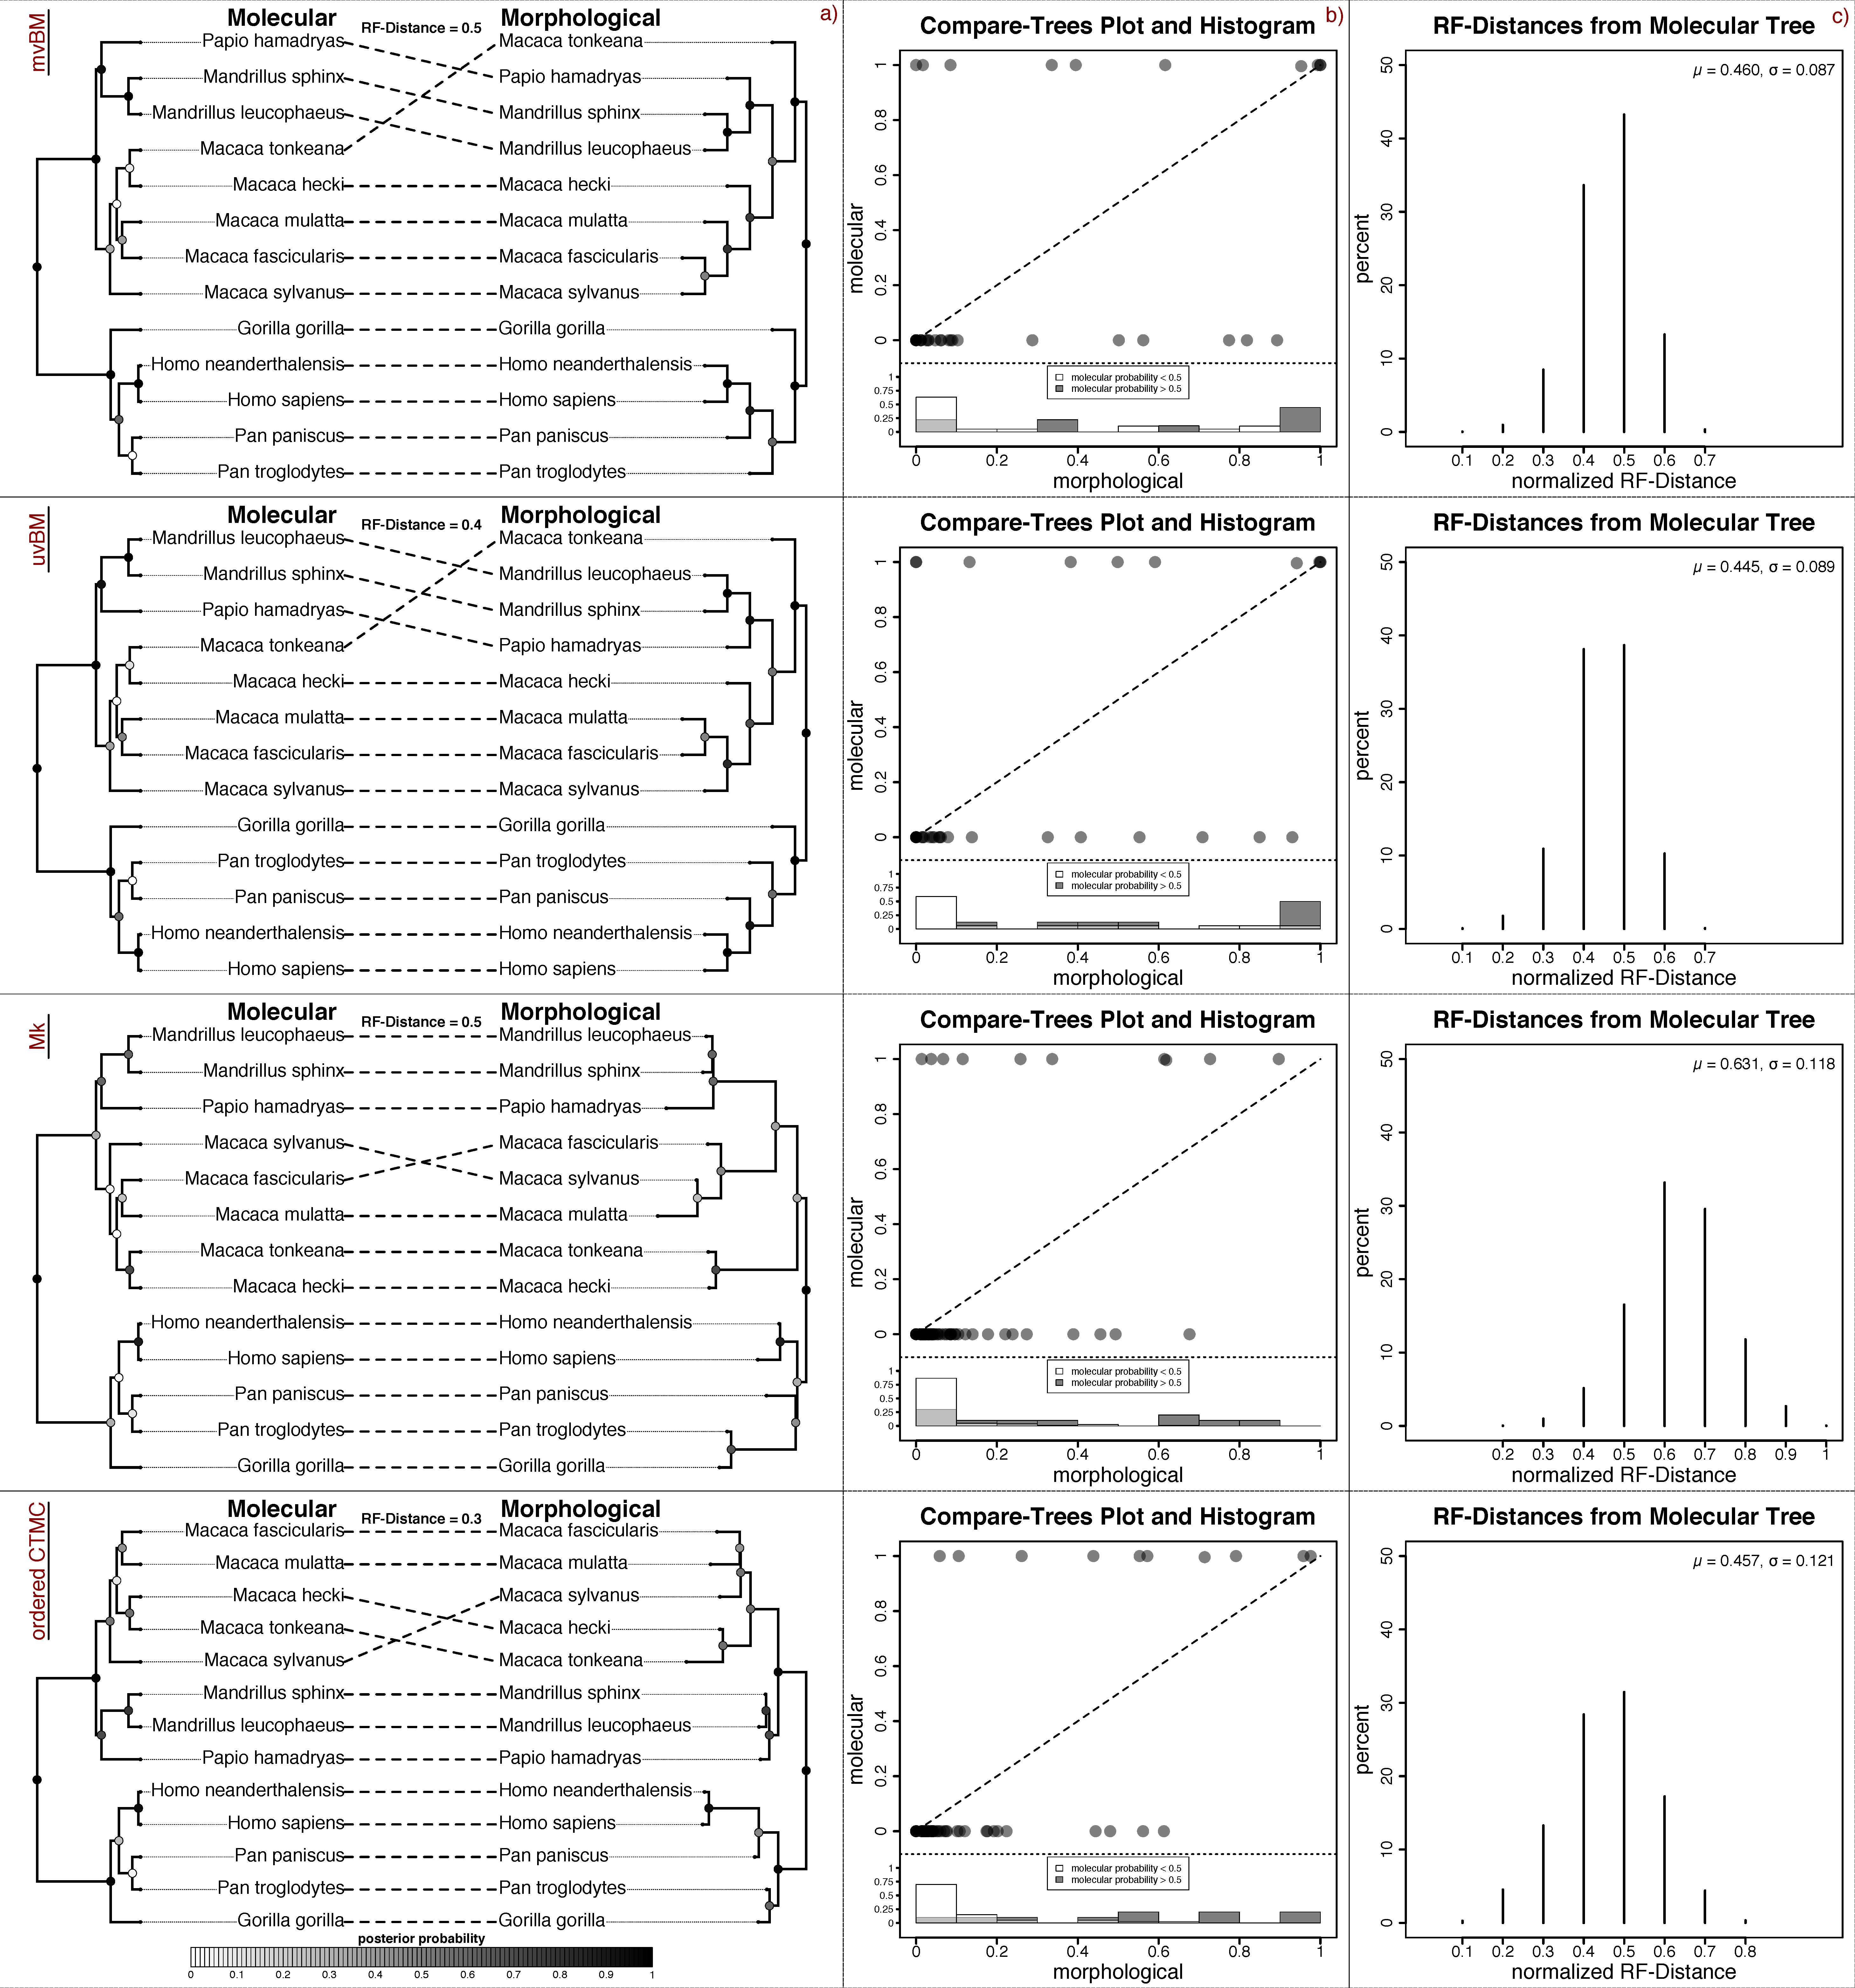
\includegraphics[width=160mm]{figures/harvati_figure1_final.pdf}
\caption[Visualizing Results of Model-Based Phylogenetic Analyses of Catarrhine Landmark Data]{In a), cophylo plots of molecular MCC trees opposing those from the four morphological analyses specified above. In cophylo plots, nodes of two opposing trees are rotated as to match tips along the vertical dimension. Both trees were rooted using cercopithecoids as an outgroup. Nodal posterior probabilities from the morphological analyses are marked along a white-to-black gradient. In b), compare-trees plots of bipartition probabilities from the morphological analyses (horizontal axis), and from the 10kTrees Project trees. Histograms of bipartitions from the morphological analyses appear in the lower portion of the graph. In c), normalized Robinson-Foulds distances from the morphological posterior distributions to the Molecular MCC tree.  \label{overflow}
\label{fig:harvatiFigure1}}
\end{figure*}

\begin{figure*}[h]
\centering
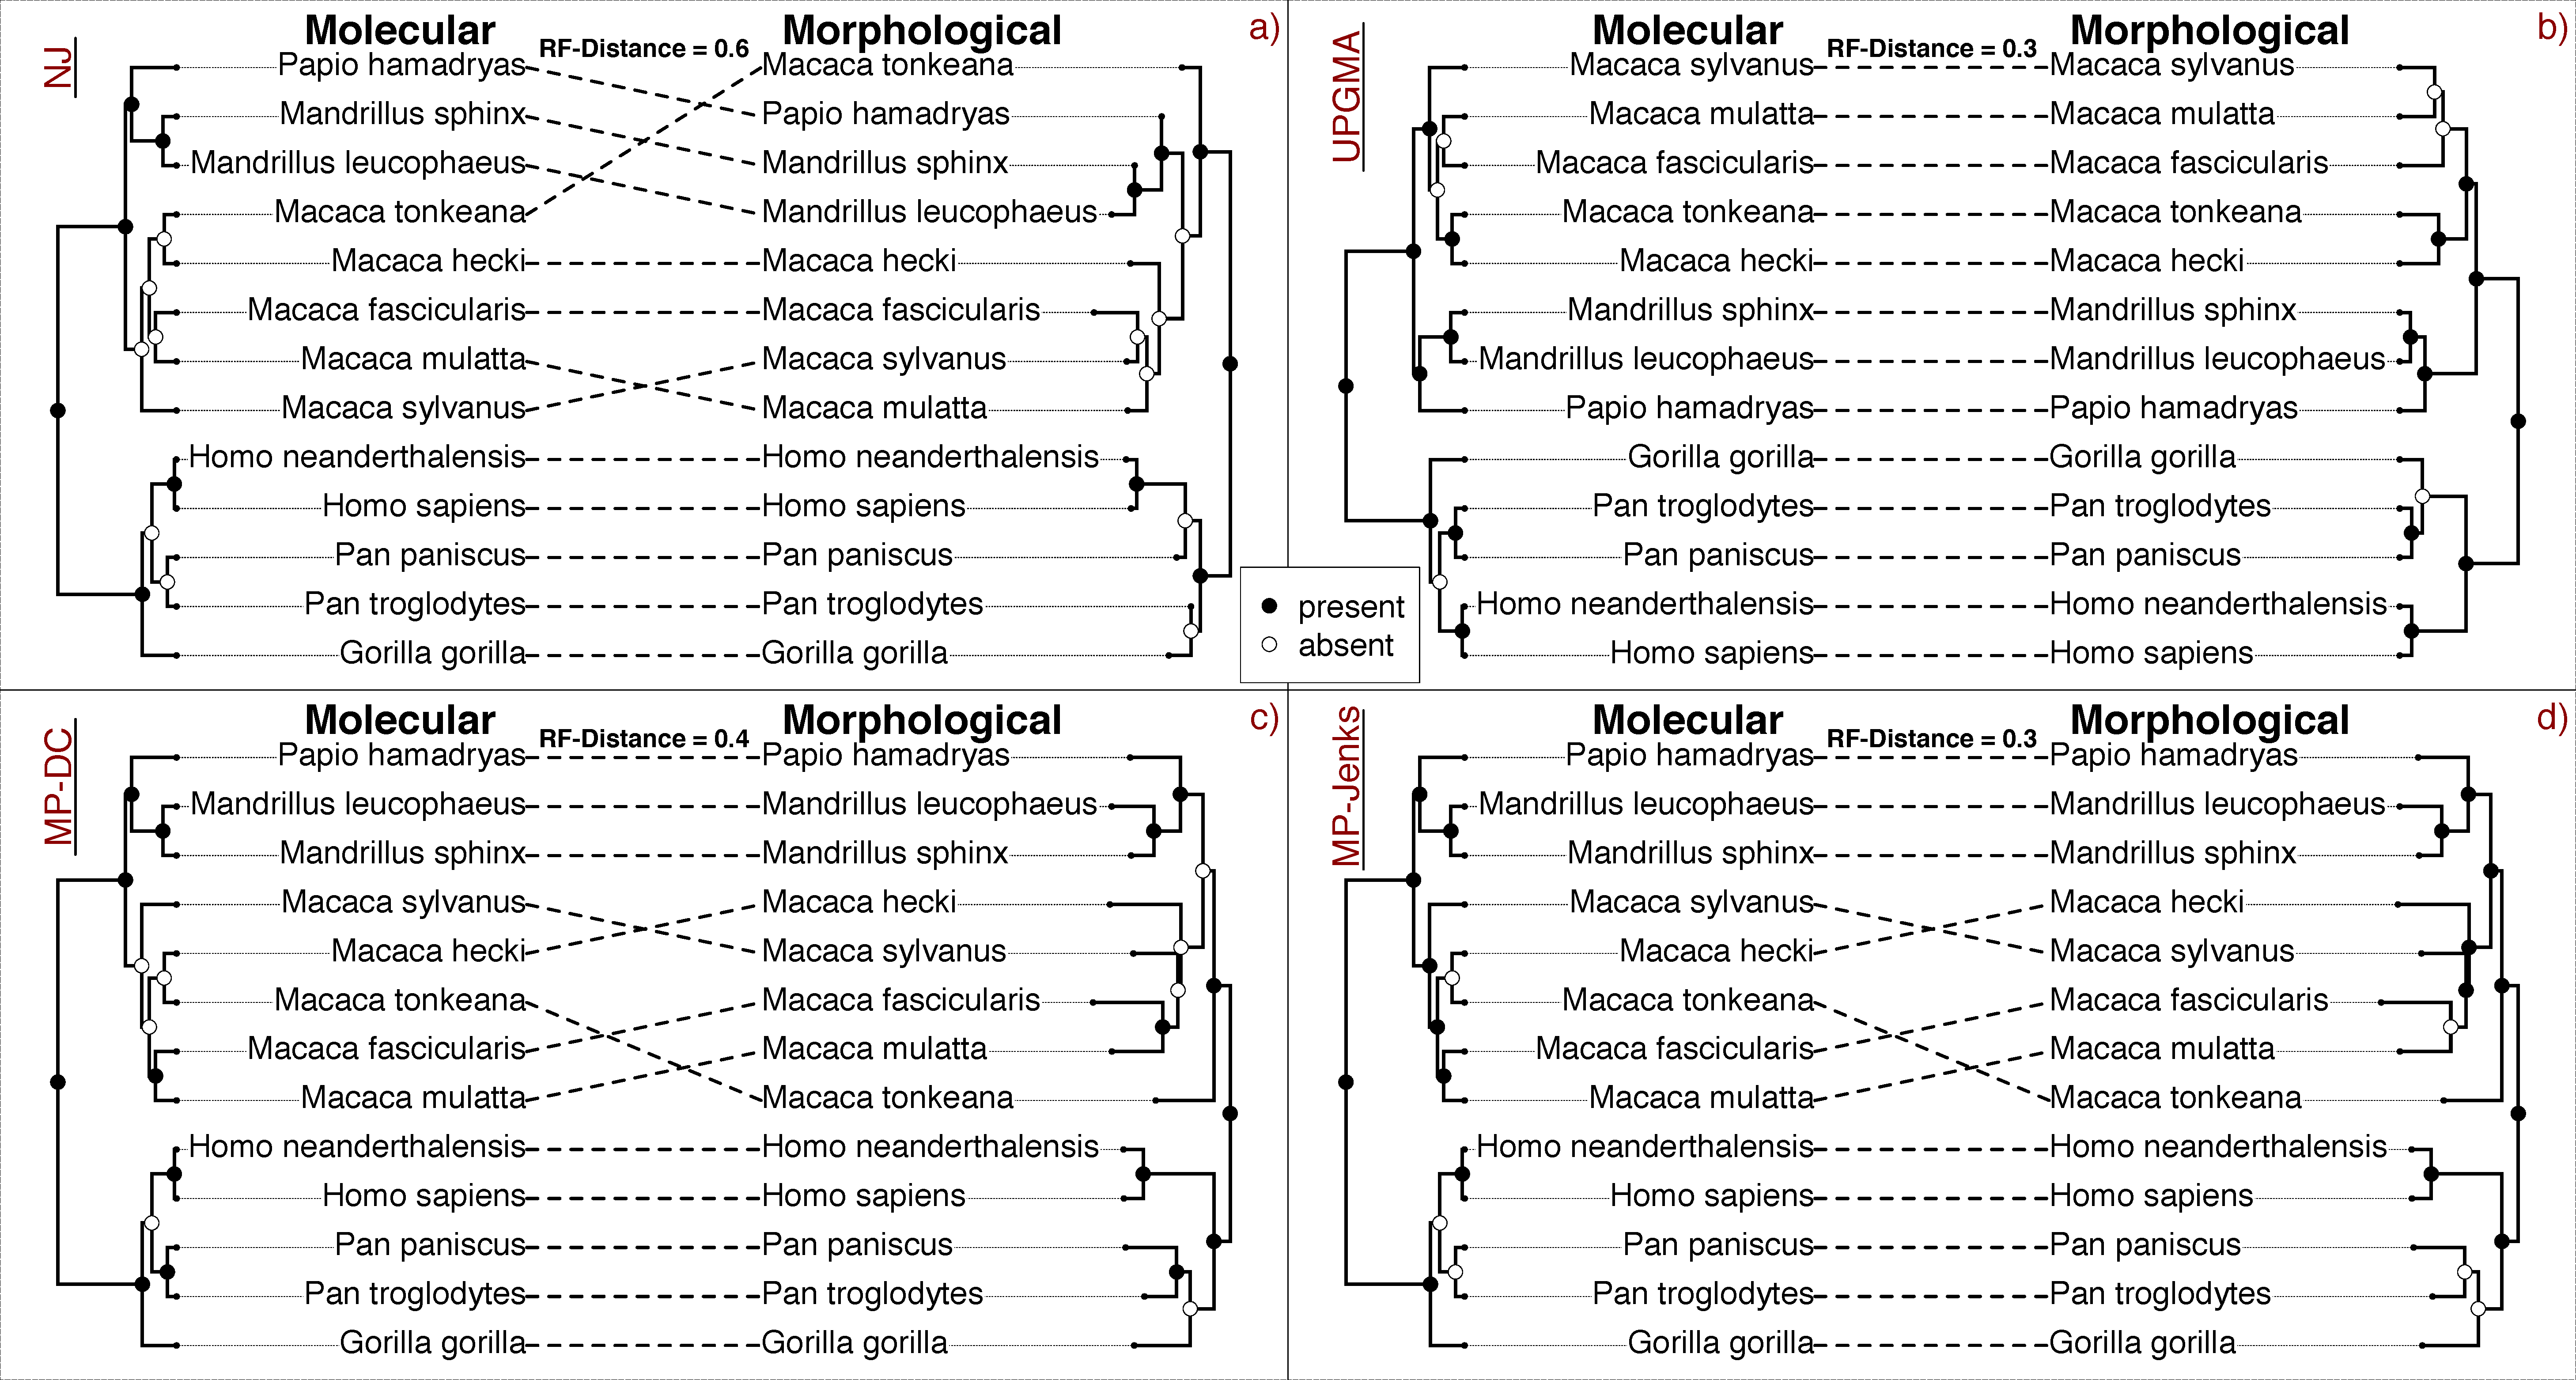
\includegraphics[width=160mm]{figures/harvati_figure2_final.pdf}
\caption[Visualizing Results of Heuristic Phylogenetic Analyses of Catarrhine Landmark Data]{Cophylo plots of molecular MCC trees opposing those from the four morphological analyses specified above, with normalized Robinson-Foulds distances shown. Here, each of the morphological trees produced only point estimates, so nodes are marked according to bipartition presence and absence in the opposing tree. In a), the neighbor-joining tree is shown. In b), the UPGMA tree. In c), the maximally parsimonious tree obtained from PC scores discretized using divergence coding. And in d), the maximally parsimonious tree obtained from PC scores discretized using the Jenks Natural Breaks algorithm with 4 expected categories. \label{overflow}
\label{fig:harvatiFigure2}}
\end{figure*}

\begin{figure*}[h]
\centering
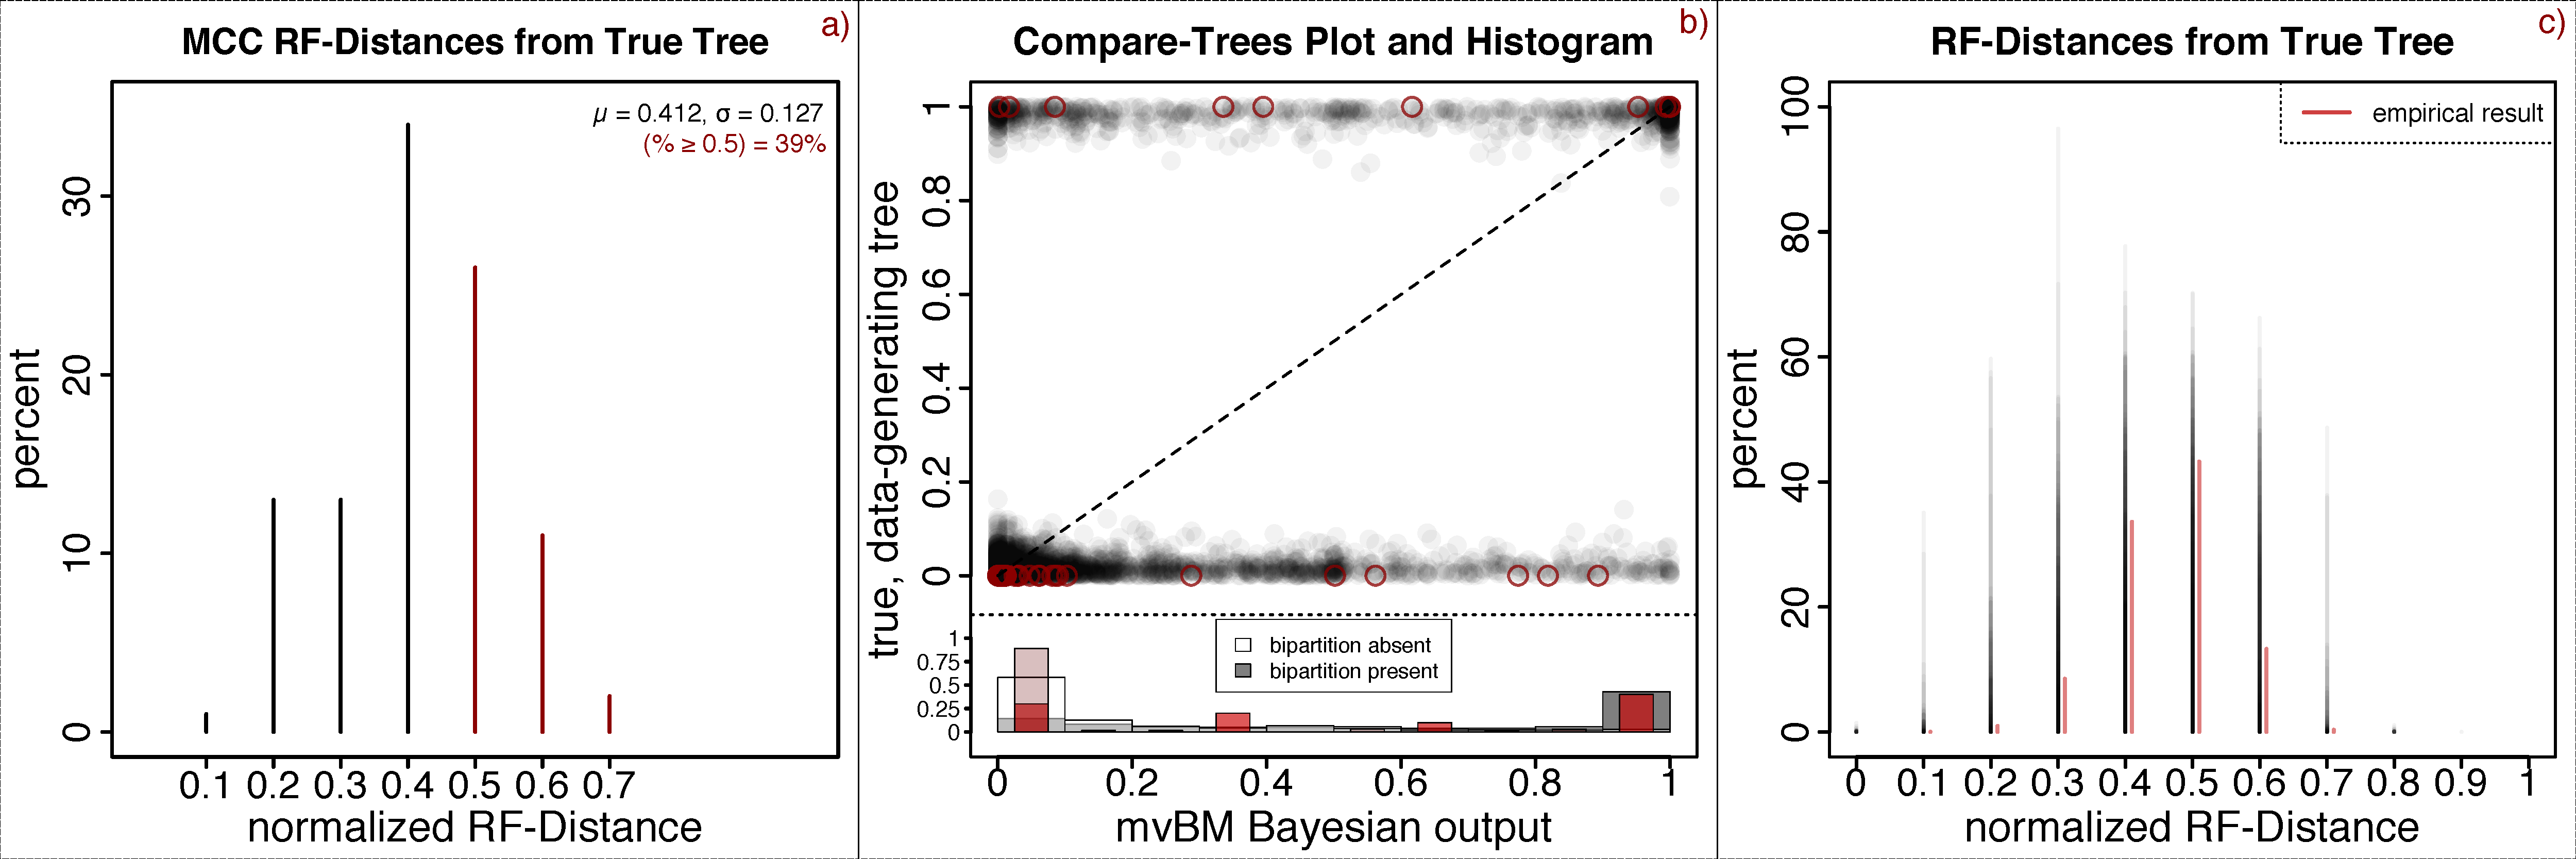
\includegraphics[width=160mm]{figures/harvati_figure3_final_redo.pdf}
\caption[Visualizing Results of Empirically Parameterized Simulation Study Relative to Empirical Result]{In a), we see the distribution of normalized RF-distances of the Bayesian MCC tree from the true, data-generating tree across the 100 replicates of our simulation experiment. The mean and standard deviation of this distribution are given, with distances greater than or equal to our empirical mvBM distance from the molecular tree (0.5) marked in dark red. In b), we construct similar plots across simulation replicates as in figure 1b, jittering probabilities inwards to better represent simulation variance. In the bottom section of the plot, two histograms of the average (across replicates) posterior bipartition probabilities are constructed, one corresponding to bipartitions that are present and the other to bipartitions that are absent. As in a), the empirical result is marked in red. In c) we visualize the distribution of RF-distributions from the data-generating tree across simulation replicates, depicting also the empirical result for each normalized RF-distance to the right of the corresponding simulation result. \label{overflow}
\label{fig:harvatiFigure3}}
\end{figure*}

\begin{figure*}[h]
\centering
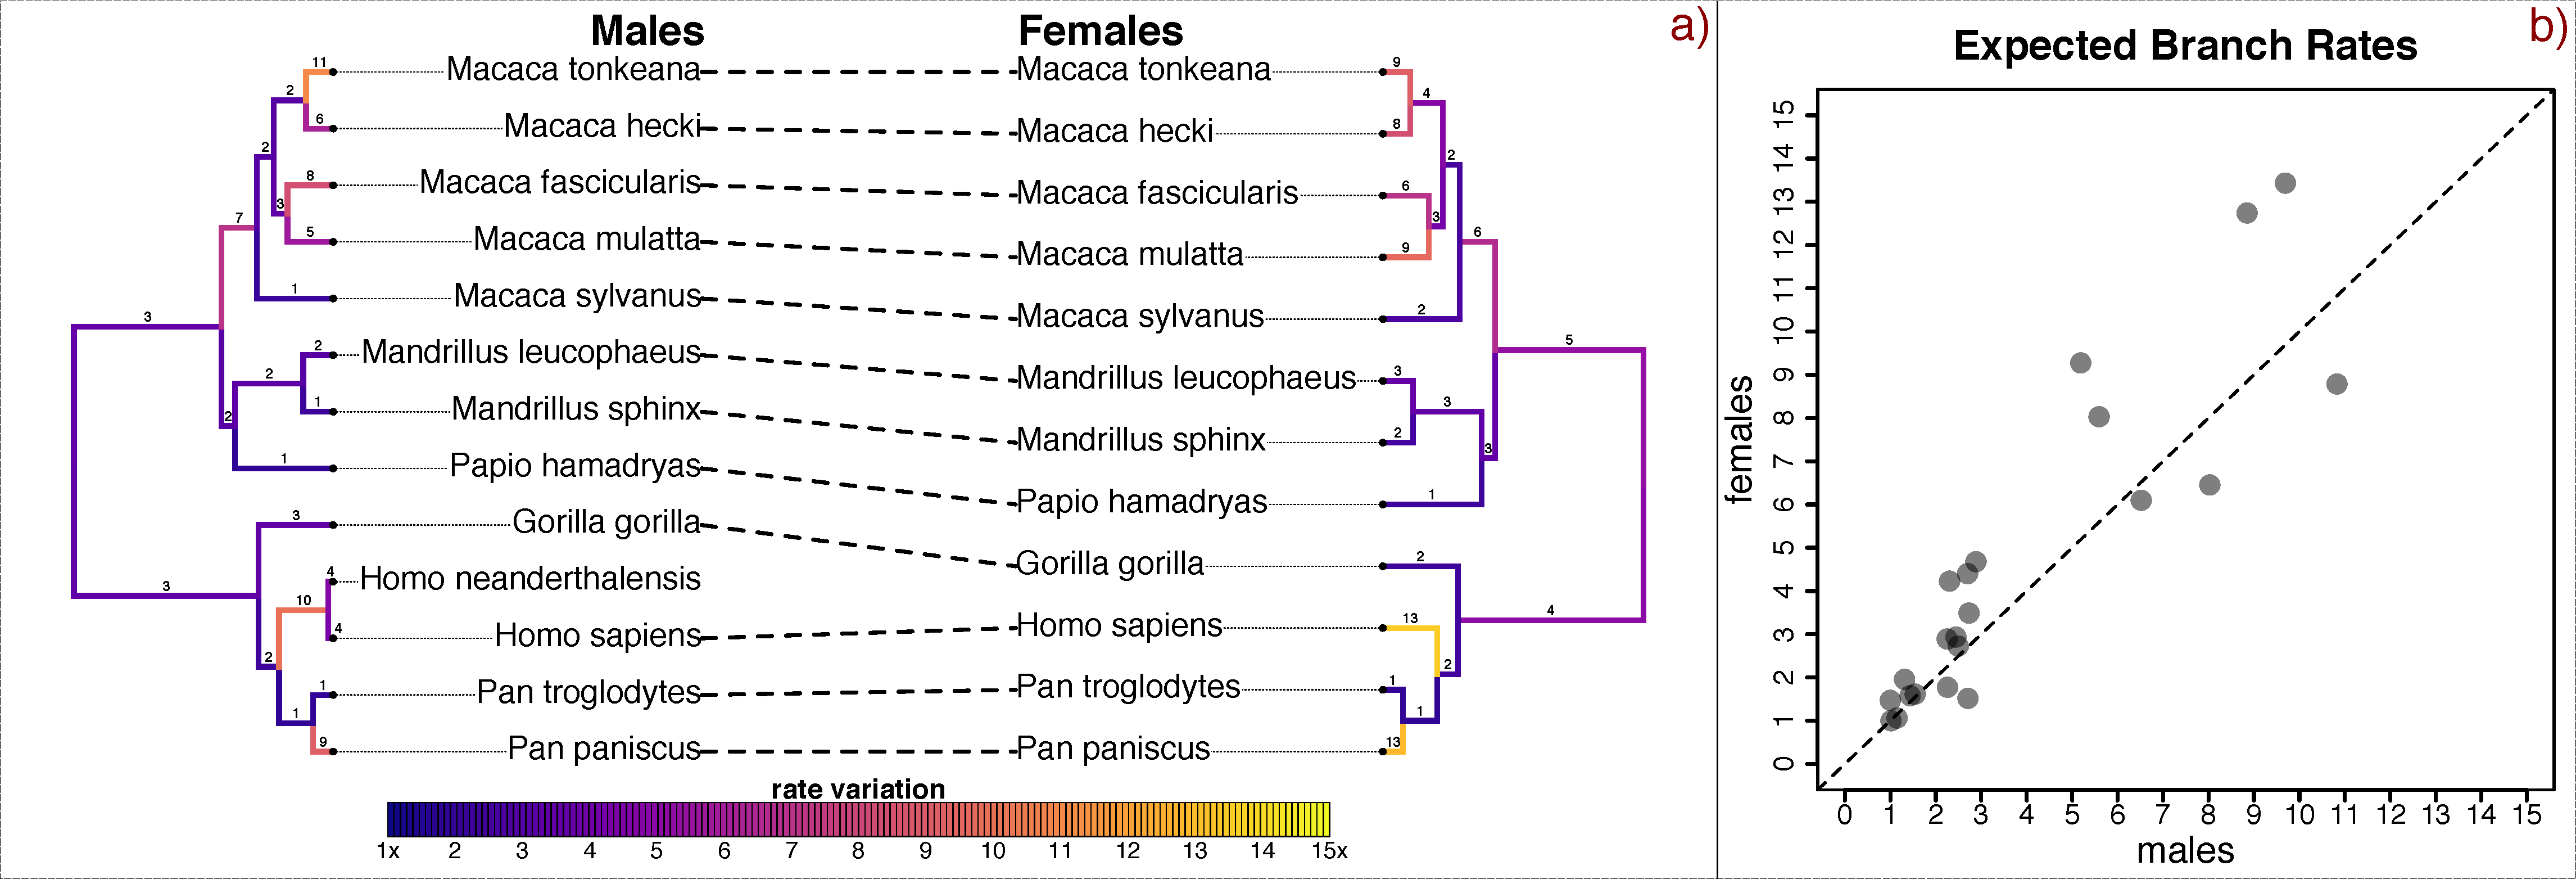
\includegraphics[width=160mm]{figures/harvati_figure4_final.pdf}
\caption[Rate Variation in Catarrhine Cranial Evolution]{In a), cophylo plots of molecular MCC trees with male and female mean branch rates colored according to the heatmap at the bottom of the figure and labeled above each branch. Branch rates arithmetically average over the Bayesian marginal posterior, discarding inferential uncertainty. To allow rates to be compared on a common scale, male and female branch rates were divided by the slowest branch rate in their respective partition, in both cases corresponding to the branch subtending the cercopithecoids. We more directly compare these branch rates in b), where relative branch lengths are plotted for both partitions. As the female tree lacked a Neandertal tip, we matched the branch rate of the branch subtending the Neandertal-\textit{Homo sapiens} MRCA in the male tree to the terminal \textit{Homo sapiens} branch of the female tree, to better reflect the cranial differentiation present along the hominin lineage after its split from that of the chimpanzee. \label{overflow}
\label{fig:harvatiFigure4}}
\end{figure*}

\begin{figure*}[h]
\centering
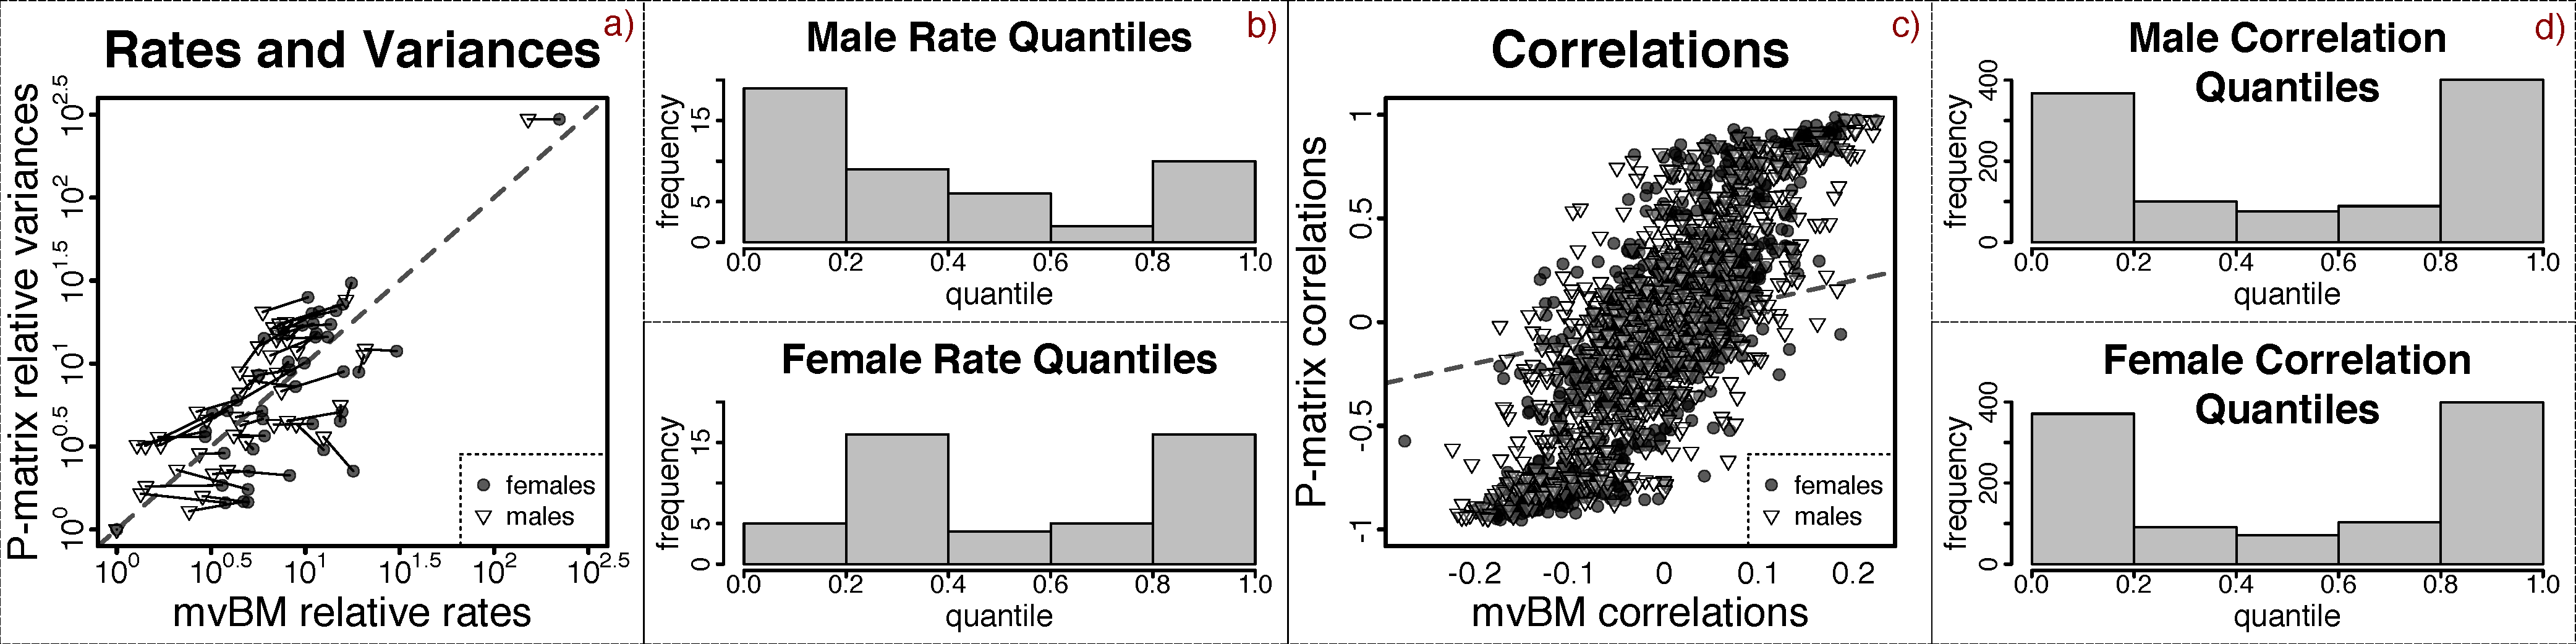
\includegraphics[width=160mm]{figures/harvati_figure5_final.pdf}
\caption[Evaluating Cheverud's Conjecture: Does an Inferred Rate Matrix Resemble Within-Group Patterns of Variation and Covariation?]{In a), a scatter plot of posterior mean trait-specific rates of evolution on the horizontal axis and pooled within-group phenotypic variances on the vertical axis. Males and female estimates for the same trait are connected by thin solid line black lines, and the 1-to-1 line is shown by a dashed line. For these to be comparable on a common scale, both were standardized by dividing all rates by the smallest rate, which in both sets corresponded to the same coordinate (the $Z^{th}$ position of the $7^{th}$ landmark). Rescaling the entire marginal posterior by each sample-specific instance of this value, in b) we depict the distribution of quintiles into which the rescaled pooled within-group variance for each trait fell. In c), we compare posterior mean pairwise correlations with their corresponding pooled-within group (P) correlations, once more drawing a dashed 1-to-1 line. In d), the distribution of quintiles of each pairwise P correlation in their matched marginal posterior distribution is shown.  \label{overflow}
\label{fig:harvatiFigure5}}
\end{figure*}

\begin{figure*}[h]
\centering
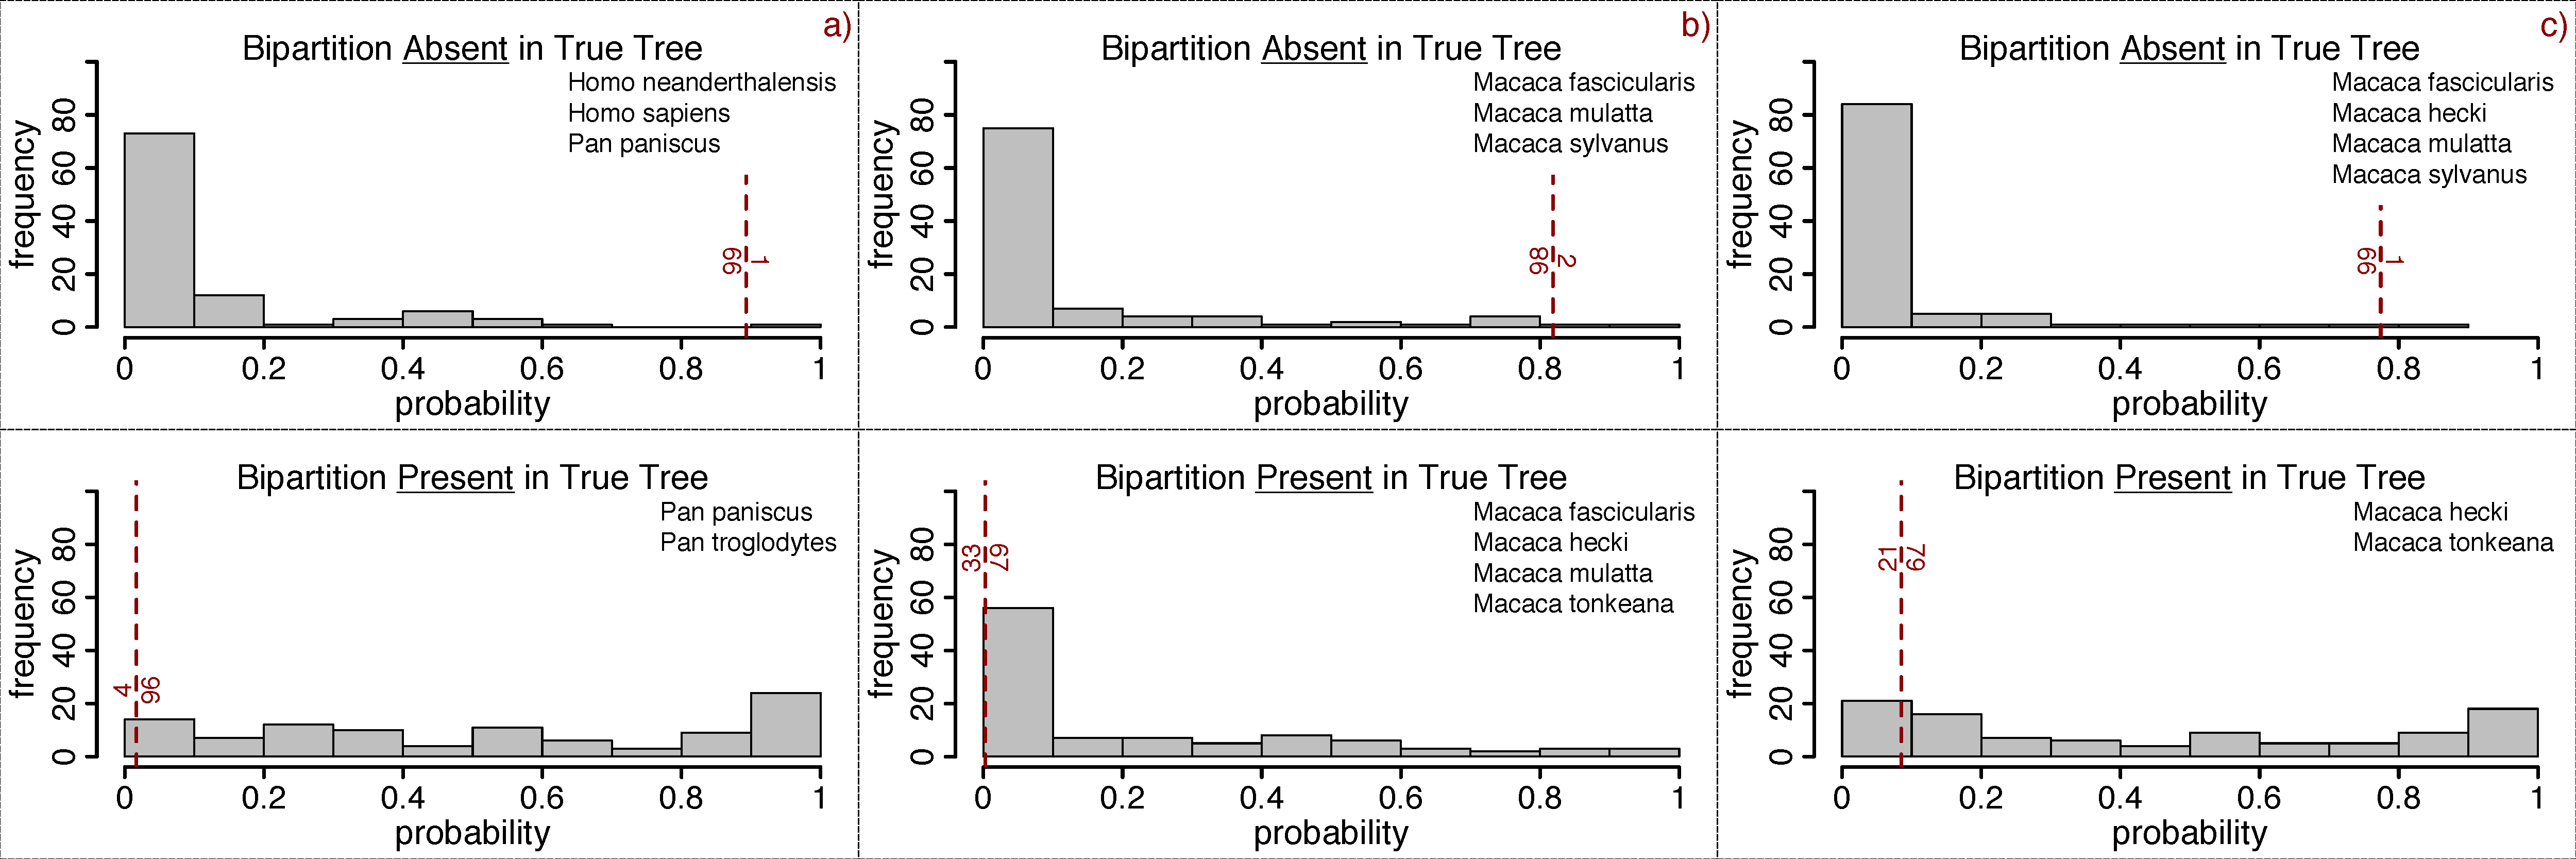
\includegraphics[width=160mm]{figures/harvati_figure6_final_redo.pdf}
\caption[Querying the Simulation Experiment for Concordance in Phylogenetic Error]{Each panel corresponds to a \textit{fractious} bipartition in the empirical tree whose estimated probability in the mvBM morphological analysis was $>0.75$ away from the corresponding bipartition's molecular probability. The morphological probability is marked by a dark red vertical line, and the histograms represent that bipartition's probability across the 100 replicates of our simulation experiment. Numbers on either side of the dashed line represent the proportion of simulated runs falling on either side. The set of taxa comprising the bipartition is given in the upper right-hand corner of each panel. Presence and absence of particular bipartitions in the tree can be paired, as all trees are strictly bifurcating and one mismatch necessarily implies another. As such, we have organized the figure into three P/A pairs, labeled \textit{a)}, \textit{b)}, and \textit{c)}. \label{overflow}
\label{fig:harvatiFigure6}}
\end{figure*}

%\begin{figure*}[h]
%\centering
%\includegraphics[width=160mm]{figures/harvati_figure7_final.pdf}
%\caption{ blah blah blah
%\label{overflow}
%\label{fig:harvatiFigure7}
%}
%\end{figure*}


\clearpage

\section{Tables}

% latex table generated in R 3.6.2 by xtable 1.8-4 package
% Mon Nov 23 17:25:41 2020
\begin{longtable}{rrrr}
  \hline
 & Males & Females & Total \\ 
  \hline
\textit{Gorilla gorilla} &  48 &  36 &  84 \\ 
  \textit{Homo neanderthalensis} &   5 &   0 &   5 \\ 
  \textit{Homo sapiens} & 118 & 112 & 230 \\ 
  \textit{Macaca fascicularis} &  30 &  21 &  51 \\ 
  \textit{Macaca hecki} &  10 &   7 &  17 \\ 
  \textit{Macaca mulatta} &  11 &  12 &  23 \\ 
  \textit{Macaca sylvanus} &  10 &  10 &  20 \\ 
  \textit{Macaca tonkeana} &   9 &  11 &  20 \\ 
  \textit{Mandrillus leucophaeus} &  22 &  15 &  37 \\ 
  \textit{Mandrillus sphinx} &  19 &  12 &  31 \\ 
  \textit{Pan paniscus} &  21 &  28 &  49 \\ 
  \textit{Pan troglodytes} &  55 &  74 & 129 \\ 
  \textit{Papio hamadryas} & 264 & 136 & 400 \\ 
   \hline
\hline
\caption[Composition of Landmark Data Used in Empirical Analysis]{A table detailing the composition of the landmark dataset used in 
                                            our empirical analysis. Elements of the table represent numbers of individuals in each 
                                            row species corresponding to each 
                                            estimated column sex. Further details regarding landmarks used can be found in \citep{harvatiNeanderthalTaxonomyReconsidered2004}.} 
\label{tab:landmarkDataComposition}
\end{longtable}
